\section{Formative Work: Understanding Creative Live Streams}
\label{sec:liveclips_formative}
Creative live streams are a unique and rapidly growing source of data that have yet to be deeply studied.  To understand the current landscape of creative live streams as well as their applicability to inspiration in software, we conducted content analysis and surveys, exploring the following two questions:

\begin{enumerate}
    \item \textbf{What are creative live streams?} For a general sketch of creative live streams, we present a content analysis of a sample of live streams that illustrates the range of creative content people stream and the different types of creative live streams.
    \item \textbf{Why do people watch creative live streams?} To understand the motivations behind creative live stream viewers, we present findings from three online surveys with 165 viewers that highlight learning and inspiration as key motivators.
\end{enumerate}

We found that viewers often seek to learn and be inspired from creative live streams. Notably, inspiration is a much more prominent theme compared with prior work in other live streaming domains such as gaming. However, many streaming platforms are not designed to support these goals, and watching archived streams is tedious. These findings further motivate our goal to make creative live streams available to users in the context of their own workflows.

We were also interested in streamers' experiences producing creative live streams, so we conducted interviews with 8 streamers. These interviews did not directly inform the design of LiveClips as it does not address the streamer's experience, but our findings provide useful insights that future work may build on towards improving the creative streamer's experience. Appendix \ref{chapter:appendix} reports our interview methodology and findings in detail.

\subsection{What Are Creative Live Streams?}
Live stream videos (\autoref{fig:livestreaming_view}) typically show the artist's full screen (when working on a computer) or workspace (for physical work) and a camera view of their face. Live streams usually also feature a live chat, allowing viewers to communicate with each other and the artist. 

\begin{figure}[b!]
\centering
  \includegraphics[width=0.7\columnwidth]{liveclips/figures/livestreaming_paper_figure_anonymized.jpg}
  \caption[A typical creative live stream setup.]{A typical creative live stream setup. (a) A camera or screencast displays the artist's workspace. (b) A second camera shows the artist's face, usually via their computer's webcam. (c) Graphical overlays provide ambient information about the artist (\textit{e.g.}, social media pages) and display interactions with the audience (\textit{e.g.}, pop-ups that appear when viewers subscribe or donate to the stream). (d) Live chat allows viewers to communicate with the streamer. }~\label{fig:livestreaming_view}
\end{figure}

There are two main things that make live streamed videos different from other types of videos demonstrating creative work, such as tutorials. First, live streamed videos usually show a real-world process, imparting both creative and procedural knowledge, while tutorials often show contrived tasks, and impart mainly procedural knowledge \cite{Torrey2007}. Second, artists often start without an exact goal in mind, and it can be inspiring to watch someone go from a blank canvas to a beautiful piece of work, though this also means watching the less ``glamorous'' parts of the creative process such as silent thinking or tedious, repetitive tasks.

To learn more about creative live streams, we studied two popular platforms: Twitch and YouTube. As these large platforms cover many types of content, we narrowed our investigation to the \textit{Creative} category on Twitch and the \textit{Adobe Live} video series on YouTube. Through this, we see how streams and communities differ across platforms. Our findings also inform the design and implementation of LiveClips, which uses videos from these same two categories as its corpus for extracting short inspirational clips.

\subsubsection{Creative live streams on Twitch: Content analysis}
To better understand the format and content of creative live\-streams, we analyzed a sample of videos on Twitch, one of the most popular platforms for live streaming. Twitch launched its \textit{Creative} category in 2015 \cite{Moorier2015}. To deal with its explosion in popularity, Twitch replaced the \textit{Creative} category with six more-specific categories in September 2018: \textit{Art}, \textit{Music \& Performing Arts}, \textit{Science \& Technology}, \textit{Beauty \& Body Art}, \textit{Food \& Drink}, and \textit{Makers \& Crafting} \cite{Robertson2018}. For each category, we gathered aggregate metrics about streamers and viewers. We watched and took notes on a sample of 29 videos. We identified four common types of creative live streams that will appear throughout the chapter: \textit{Teaching}, \textit{Making}, \textit{Socializing}, and \textit{Performing}.

Although the current LiveClips system focuses on digital creative work, the platforms we analyzed include streams of both digital and physical work. This provides a more comprehensive look at the general creative live streaming space, to inform both LiveClips and other future work on creative live streaming.

\textbf{Methodology:}
To measure the popularity and activity in each of the six creative categories, we queried the Twitch \textsc{api} 4 times a day for 7 days to obtain the number of currently-live streams and number of currently-watching viewers in each category.

We also used the Twitch \textsc{api} to download metadata about the videos in each category (limited to top 600)
%Because this \textsc{api} halts video requests after 600 videos, so our script downloaded metadata for the 600 most-viewed videos in each category. The script 
and randomly selected 50 archived English live stream videos. Four annotators (including the first author) watched each of these videos. Ten videos were not available for viewing and thus excluded (either because their archive expired between being downloaded and being annotated, or because they were only available to subscribers of a channel). Another 11 videos were excluded as they showed video games, TV show reruns, or live event coverage. While these videos were categorized as creative on Twitch, they did not reflect our definition of creative work, namely the creation of a novel artifact. This yielded 29 videos. For each, annotators took notes in a structured spreadsheet on the content presented, camera setup, overall structure of the stream, artist's presentation style, and chat activity.

\begin{table}[t]
\centering
\caption{Summary of popularity of Twitch's creative live stream categories. The number of currently-live streams and currently-watching viewers were collected 4 times a day for a week and then averaged.}~\label{table:livestream_summary}
\resizebox{0.7\textwidth}{!}{
\begin{tabular}{llll}
\textbf{Category}        & \textbf{\begin{tabular}[c]{@{}l@{}}Avg. \#\\ live streams\end{tabular}} & \textbf{\begin{tabular}[c]{@{}l@{}}Avg. \# live\\ viewers\end{tabular}} & \textbf{\begin{tabular}[c]{@{}l@{}}Avg. \# viewers\\ / stream\end{tabular}} \\
Art                      & 339                                                                    & 6417                                                                    & 21                                                                          \\
Beauty \& Body Art       & 5                                                                      & 177                                                                     & 17                                                                          \\
Food \& Drink            & 19                                                                     & 1088                                                                    & 64                                                                          \\
Makers \& Crafting       & 40                                                                     & 680                                                                     & 16                                                                          \\
Music \& Performing Arts & 286                                                                    & 6881                                                                    & 24                                                                          \\
Science \& Technology    & 91                                                                     & 1155                                                                    & 12                                                                         
\end{tabular}
}
\end{table}

%While this sample does not capture all types of creative activities one might live stream, our hope is that by analyzing a set of canonically creative activities we can shed light on a broader set of activities that might also have a creative component (\textit{e.g.}, video games that involve creating artifacts).
%There is overlap among categories on Twitch, even sometimes within a single live stream when an artist switches back and forth between creative work and other activities like gaming. 

\textbf{Results: Most streamers focus on work \& engage with viewers:}
\autoref{table:livestream_summary} shows overall metrics for the creative categories on Twitch. The most popular categories by far are \textit{Art} and \textit{Music \& Performing Arts}. The category with the most viewers watching per stream is \textit{Food \& Drink}, likely because there are fewer streams to choose from relative to the number of interested viewers. These communities are small relative to the most popular games; for example, the game Fortnite has between 5,000 and 10,000 streams live on Twitch at any given time, with around 100,000 total viewers watching. %\xxx{xxx says move earlier but where?}

\begin{table}[t!]
\centering
\caption{Creative activities shown in a random sample of 29 live streams from Twitch's creative categories, and the primary type of structure each stream exhibits.}~\label{table:livestream_activities}
\resizebox{0.7\textwidth}{!}{
\begin{tabular}{lll}
\textbf{Category}        & \textbf{Activity (\# videos if \textgreater 1)} & \textbf{\begin{tabular}[t]{@{}l@{}}Primary type\\ of stream\end{tabular}} \\
Art                      & Multimedia production                           & Making                                                                    \\
                         & Digital drawing (4)                             & Making                                                                    \\
                         & Animation                                       & Teaching                                                                  \\
                         &                                                 &                                                                           \\
Beauty \& Body Art       & Makeup                                          & Socializing                                                               \\
                         & Makeup (3)                                      & Making                                                                    \\
                         &                                                 &                                                                           \\
Food \& Drink            & Cooking                                         & Teaching                                                                  \\
                         &                                                 &                                                                           \\
Makers \& Crafting       & Making foam props                               & Teaching                                                                  \\
                         & Sewing quilts                                   & Socializing                                                               \\
                         & Bead art (2)                                    & Making                                                                    \\
                         & Assembling models                               & Making                                                                    \\
                         & Assembling models                               & Socializing                                                               \\
                         & Woodworking                                     & Making                                                                    \\
                         & Pottery                                         & Making                                                                    \\
                         &                                                 &                                                                           \\
Music \& Performing Arts & Music production                                & Performing                                                                \\
                         & Music production                                & Making                                                                    \\
                         & Acting \& improv games                          & Performing                                                                \\
                         &                                                 &                                                                           \\
Science \& Technology    & Building a computer                             & Making                                                                    \\
                         & Programming (3)                                 & Making                                                                    \\
                         & Game development (2)                            & Teaching                                                                  \\
                         & Talking about technology                        & Socializing                                                              
\end{tabular}
}
\end{table}

The videos span a range of creative activities (\autoref{table:livestream_activities}). The average video length was 3h46m, not including time spent gaming -- a few artists combined both creative work and video gaming into one stream, spending the first part on creative work then switching to gaming when they were finished. The shortest video was 1h3m; the longest was 7h56m. These videos are notably longer than most non-live-stream videos, which are already difficult to browse and navigate \cite{Chi2012, Pongnumkul2011, Nguyen2015}. This further motivates LiveClips' goal of extracting shorter clips, as a multi-hour-long video is not likely to be helpful in context while the user is working.

Almost all videos contained either a screencast view for work being done on a computer (13/29) or a camera view for physical work (15/29). One showed a distant camera view of the artist producing music in a studio. Most (26/29) showed the artist's face: in 10 as part of the main camera feed, and 16 as a separate feed overlaid in a corner (as in \autoref{fig:livestreaming_view}). Of the 13 videos that showed screencasts of digital work, 10 showed the artist's face overlaid in a corner and 3 did not show the artist's face at all. Almost all artists (27/29) talked out loud while streaming; of the two silent streamers, one occasionally posted in the chat. Most artists talked about a mix of their work and other topics (18/29). Some talked only about their work (9), or only about other topics (1). One was a variety show, so the talking \textit{was} the work. Many videos (19/29) included background music. 

Most artists engaged with the chat at least sometimes (24/29). 18 artists engaged frequently with the chat, and 6 occasionally. Three videos did not show a chat replay despite the artist referring to the chat; we assume it was not saved or had been hidden. In all 26 remaining videos, viewers asked questions at least occasionally, or in some videos (9/26) frequently. In half of these videos, all chat questions appeared to get answered; in the rest, some (7/13) or many (4/13) questions went unanswered. In 2 videos, most chat questions were answered by other viewers or moderators in the chat.

\textbf{Four common types of creative live streams:}
We identified four common types of creative live streams. We also observed these in our interviews with streamers (see Appendix \ref{chapter:appendix}). Sj{\"{o}}blom \textit{et al.} \cite{Sjoblom2017a} offer a similar characterization of video game live streams; we found some key differences and fewer overall types of structures. \autoref{table:livestream_activities} shows the primary type of each stream in our sample set. These are general high-level trends; some streams bridge multiple types.

\textbf{Teaching} streams have an instructional focus, where the stream\-er is educating the viewers. These include step-by-step how-to demonstrations of tasks such as cooking a recipe, producing a photo-editing effect, or creating DIY costumes. Other examples include critiquing others' work, answering viewers' questions, or explaining a topic.

\textbf{Making} streams focus primarily on creative work and process, but not explicit teaching. These include an artist silently drawing, a streamer attempting a new task they have not tried before and talking their way through it, and an artist making pottery and describing \textit{what} they are doing but not \textit{how}. 

\textbf{Socializing} streams feature the streamer chatting casually with viewers, often while working on a project, such as makeup or sewing (but the project is not the main focus). These are often described as ``chill'' streams. Socializing streams often have tight-knit communities; the streamer will recognize the names of viewers in the chat and ask them how they are doing.

\textbf{Performing} streams feature the artist performing their work. Naturally, these mostly include performative arts like music and acting (\textit{e.g.}, as opposed to drawing). Like with Making, the focus is on the artist's work; in this case the artist does not talk about what they are doing, they just do it. Performing streams differ from non-live recordings in that they often take a more casual improvisational form, rather than scripted performance (\textit{e.g.}, musical ``jam sessions'' or improv acting).

Within each type, the amount of interaction between the stream\-er and the audience varies. Some streamers hold ``request streams'' or ``Q\&A streams'', where the content and flow are determined by audience requests or questions, respectively. Some hold contests or games. A request stream could have audience members requesting songs for a Performing stream, a topic for a Teaching stream, or a particular artifact for the artist to make in a Making or Socializing stream. Finally, as \autoref{table:livestream_activities} shows, the majority of live streams showing digital creative activities (\textit{e.g.,} digital drawing, programming) were Making streams, and the rest were Teaching streams. Accordingly, LiveClips focuses on Making streams as its video corpus, though we believe our approach could extend to other stream types as well.

\subsubsection{Creative live streams go professional}
While many live streams are run by individuals, professionally-run streams are also growing in popularity. Adobe, a company that produces creative software, hosts live streams on a regular schedule multiple times a week\footnote{\href{https://behance.net/live}{\nolinkurl{behance.net/live}}}. These can be viewed on Behance or on Adobe's Creative Cloud YouTube channel. They host two live stream series: \textit{Adobe Live} is a Making stream that happens for 6 hours (three 2-hour sessions) three days a week, and it features guest artists usually hosted by someone who works at Adobe. \textit{Daily Creative Challenges} is a Teaching stream that happens for 30 minutes five days a week. It complements contests organized by Adobe to teach new skills. YouTube reports these streams having between 2,000 and 8,000 views each; it does not distinguish between live and replayed views.

\stepcounter{footnote}
\begin{figure}[b!]
\centering
  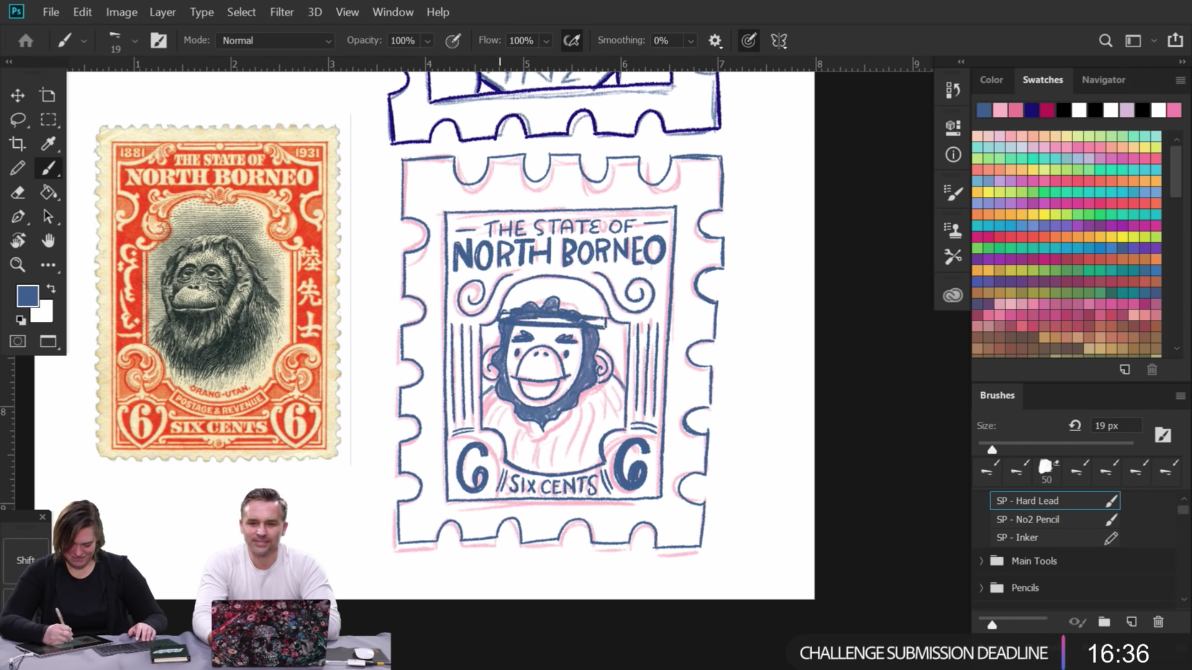
\includegraphics[width=0.6\columnwidth]{liveclips/figures/adobelive.png}
  \caption{The \textit{Adobe Live} series features a guest artist (bottom left) and a host (bottom right). The artist is working on a digital drawing, and the host is looking up at the live chat feed, engaging with the audience (\href{https://youtu.be/yYDmQhg_1uE}{\nolinkurl{youtu.be/yYDmQhg_1uE}}). }~\label{fig:livestream_adobelive}
\end{figure}

\textit{Adobe Live} differs from most streams by featuring two people. Typically there is a host and an guest artist (\autoref{fig:livestream_adobelive}), but sometimes two artists work together. Adobe hosts different artists every week across a range of creative disciplines (\textit{e.g.}, graphic design, UX design, photography, video editing). Typically, the host moderates the stream, responding to chat messages and passing on questions from viewers to the artist so that the artist can focus on their work. When the stream includes two artists, they trade off hosting.
%xxx: removing for now because we haven't talked about challenges for streamers yet
%These live streams address some of the challenges self-streamers often face, such as facilitating the chat while working and dealing with technical setup, by having separate people take on those tasks. 
The featured artists are usually practitioners, not teachers; their work mainly serves as inspirational demonstrations, while also giving the the community a chance to engage with questions and comments. 

%The \textit{Daily Creative Challenges} series features one person who both reads chat messages and provides a short tutorial on a software technique. These live streams are part of Adobe's Creative Challenges, which are contests that encourage people to use Adobe software and submit design work for prizes\footnotemark. These streams are 30 minutes long -- this is short for a live stream -- and focus on instruction: explaining the challenge of the day and teaching viewers the skill of the day. 

\footnotetext{\href{https://www.behance.net/dailycreativechallenge}{\nolinkurl{behance.net/dailycreativechallenge}}}

%The interviews and surveys in this paper are with a mix of people from Adobe's live streams and from other creative communities, allowing us to gain a broad understanding of the challenges creative streamers face and suggest possible improvements for them.


\subsection{Why do People Watch Creative Live Streams?}
To understand the motivations and challenges of creative live stream viewers, we conducted three surveys over 1.5 years with 165 people: two with \textit{Adobe Live} viewers; one with viewers of any creative live streams on the Web. All three surveys were voluntary. We found that creative live stream viewers watch streams primarily for \textit{learning} and \textit{inspiration}; community engagement and entertainment were also popular reasons for watching streams. Compared with prior work on live stream viewers in other domains, inspiration is a much more prominent theme in these survey responses. This finding motivates LiveClips' focus on contextual inspiration.
%In particular, the unique combination of learning with entertainment and engagement that live streams offer makes them an appealing choice over other types of learning-focused content.

\subsubsection{Survey methodology}
The first survey with \textit{Adobe Live} viewers (\textit{S1}) was posted periodically in the chat and overlaid on the stream for four months (August - December 2017). It asked about viewers' experience with creative software, the reasons they watch creative live streams, what other creative live streams they watch besides \textit{Adobe Live}, and how \textit{Adobe Live} streams could be improved. 98 people completed this survey.

A year later, \textit{Adobe Live} had changed considerably: more frequent streams, more audience interaction, and wider and more regular marketing. In January 2019, we conducted \textit{S2} to gain additional insights about viewer motivations and challenges, focusing especially on the live chat experience. The survey was sent directly to previous winners of Adobe's \textit{Daily Creative Challenges} who also showed up regularly in past chat logs of Adobe streams. 41 people completed this survey.

Finally, to zoom out and capture a broader range of creative live stream viewers, we conducted a third survey (\textit{S3}) with viewers of creative live streams on \textit{any}  platform. The survey was disseminated with a snowball method, via the researchers' personal social media accounts. Participants were required to have viewed creative live streams before, which were defined as ``activities such as visual art (drawing, painting, etc.), crafts, music performance, cooking, DIY projects, programming, etc.'' This survey asked viewers about the streams they watch, motivations for watching them, examples of things they learned from them, what else they do while watching, and on which platforms they watch. 26 people completed this survey.

\begin{table}[t]
\centering
\caption{All platforms listed more than once in at least one survey by respondents when asked where they watch creative live streams.}~\label{table:livestream_platforms}
\begin{tabular}{lcccc}
          & \textbf{\begin{tabular}[c]{@{}c@{}}Survey 1\\ $n=98$\end{tabular}} & \textbf{\begin{tabular}[c]{@{}c@{}}Survey 2\\ $n=41$\end{tabular}} & \textbf{\begin{tabular}[c]{@{}c@{}}Survey 3\\ $n=26$\end{tabular}} & \textbf{\begin{tabular}[c]{@{}c@{}}Total\\ $n=165$\end{tabular}} \\
YouTube   & 40                                                                 & 17                                                                 & 17                                                                 & 74                                                               \\
Twitch    & 9                                                                  & 4                                                                  & 17                                                                 & 30                                                               \\
Facebook  & 5                                                                  & 4                                                                  & 4                                                                  & 13                                                               \\
Periscope & 1                                                                  & 1                                                                  & 2                                                                  & 4                                                                \\
Instagram & -                                                                  & -                                                                  & 6                                                                  & 6                                                                \\
Phlearn   & 2                                                                  & -                                                                  & -                                                                  & 2                                                               
\end{tabular}
\end{table}

\subsubsection{What do people watch, and where?}
The most popular platform overall was YouTube (74), with Twitch second (30) (\autoref{table:livestream_platforms}). This is likely skewed by the fact that \textit{Adobe Live} is on YouTube. \textit{S3} had a smaller sample size but found YouTube and Twitch to be equally popular.

\textit{S3} respondents listed content genres they frequently watch live. Categories that came up more than once were programming (11/26), cooking (6/26), digital art (\emph{i.e.}, digital painting, photo editing) (5/26), music (4/26), physical artwork (i.e. drawing, painting) (3/26), 3D modeling (2/26), and DIY (2/26).

\subsubsection{Viewers watch for learning and inspiration}
Viewers responded similarly about motivations in all three surveys. Despite the differences in sample sizes and populations, this suggests that \textit{Adobe Live} viewers' responses may often align with viewers more broadly. Across all three surveys, learning was the most common reason people chose for watching creative live streams (\autoref{fig:livestream_survey_responses}). While learning has also been found to be an important goal for viewers in other domains such as gaming, the primary goal most often cited in prior work is entertainment \cite{Lu2019, Wohn2018, Lu2018a, Hilvert-Bruce2018, Faas2018, Cheung2011}.
%In culture-sharing live streams people learn creative skills or techniques \cite{Lu2019}. 
This difference may be due to the prevalence of Teaching live streams in creative communities.

\begin{figure}[b!]
\centering
  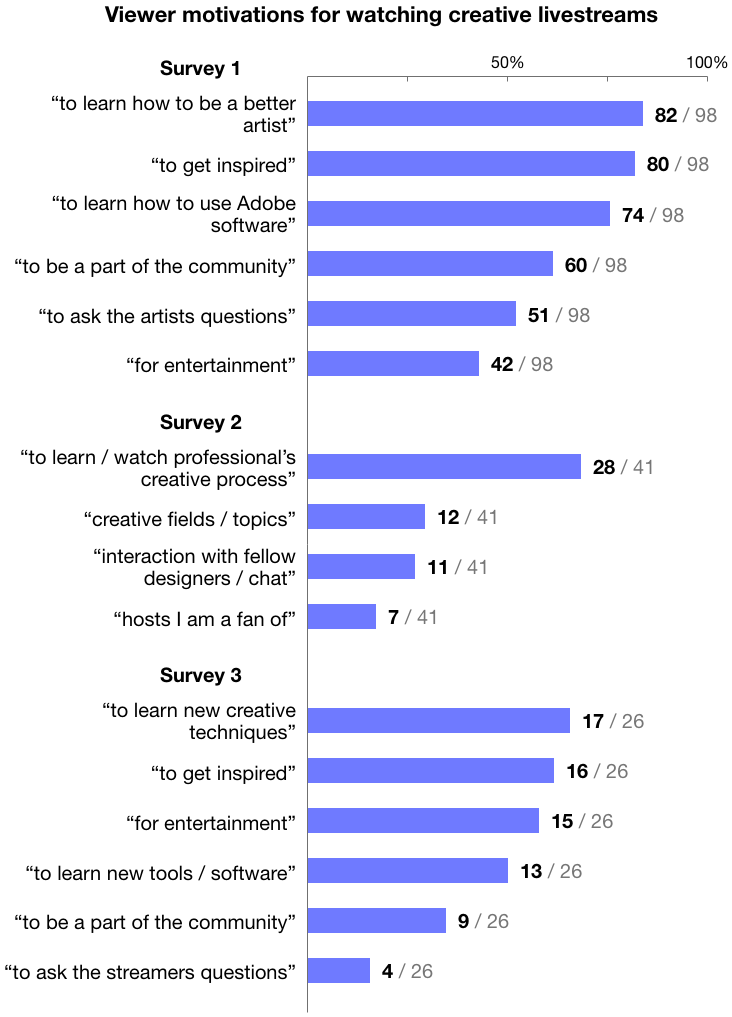
\includegraphics[width=0.7\columnwidth]{liveclips/figures/survey_responses.png}
  \caption{All three surveys asked why people watch creative live streams, allowing them to select all answers that applied from a list. This figure shows all responses chosen by at least 15\% of respondents in each survey. }~\label{fig:livestream_survey_responses}
\vspace{-0.15in}
\end{figure}

Almost all free-form elaborations on viewer motivation mentioned learning. Unlike tutorials and lecture videos, live streams offer direct interaction with the streamer and other viewers, improving the learning experience \cite{Lu2019, Faas2018}. In this way they go beyond just learning content and catalyze ``mentorship communities'' of people with similar interests \cite{Faas2018}. Learners can follow along like an apprentice in a studio, asking questions in the moment. This ability to see authentic, worked examples from start to finish reveals how the streamer makes decisions and recovers from errors \cite{Faas2018}. Viewers often use the knowledge and techniques they learn from creative live streams to inform their own work, as many \textit{S1} respondents stated in free-form responses. \textit{S3} asked for specific examples; 50\% of respondents provided one. They include adopting new techniques such as photo editing operations, trying out a streamer's creative style for things like musical playing or code commenting, and learning how to achieve a specific goal like fixing a hole in a sweater.


In addition to learning, many also reported watching for inspiration / motivation. With one exception \cite{Cheung2011}, primary work has not reported inspiration as a goal. Cheung \& Huang \cite{Cheung2011} describe ``the Inspired'' as one of nine personas for gaming live stream viewers; watching someone stream the game inspires them to play it themselves. However, a large majority of gaming stream viewers watch for entertainment, learning, or providing commentary. While inspiration can be beneficial in many genres, we believe it is especially salient in creative live streams due to inspiration's value for creative work \cite{Herring2009}.

In both \textit{S1} and \textit{S3}, inspiration was the second most popular motivation for watching creative live streams. In addition, 27\% (26/98) of \textit{S1} respondents specifically mentioned inspiration or motivation in free-form responses. 10\% (10/98) also mentioned that the videos helped increase their own motivation and confidence as artists. As one respondent explained, \textit{``[I] like watching artists work because it takes the mystery out of what they do.''} Another said, \textit{``Watching experts make mistakes gives me confidence.''}

Creative work is often a solo activity, and its nebulous nature can make it hard to stay motivated as an artist, often causing creative ``blocks'' such as writer's block. Watching someone else work can motivate viewers to keep going, as well as give them new ideas to try. Respondents in all three surveys mentioned this in free-form responses. For example, one \textit{S1} respondent said they watch live streams for \textit{``getting myself inspired and hyped before I start working.''} An \textit{S3} participant said, \textit{``It's fun seeing someone else's creative process, and usually motivates me to do my own side projects.''} LiveClips therefore explores how seeing clips from creative live streams in context might help inspire and motivate people while they work on their own creative projects.



%In \textit{S2}, 85\% of respondents said they had watched live streams of a creative activity they would not have otherwise been interested in, indicating that live streams can be a good way to discover new topics.

%not directly trying to learn but more get general creative ideas, motivate them to try their own creative projects, and inspire them to see that anyone can do creative things. 


\subsubsection{Viewers also watch for community and entertainment}
People watch all kinds of live streams for entertainment \cite{Wohn2018, Lu2018a, Hilvert-Bruce2018, Faas2018, Cheung2011}. It may be the streamer's personality or style, the chat, or the content itself. %Even though live streams may have long periods of down time with little activity, their unpredictable nature makes them ``engaging but dull'' \cite{Haimson2017}.
People also watch live streams for community. Viewers often feel emotionally attached to the streamer \cite{Wohn2018, Hu2017}, enjoy connecting and conversing with other viewers \cite{Lu2019, Lu2018, Hilvert-Bruce2018}, and enjoy being able to influence the streamer's content or process in real time \cite{Lu2018a}. Live stream communities often lead to longer-term chat groups on other platforms \cite{Lu2018a, Faas2018}.

All three surveys found community and entertainment to be secondary motivations (\autoref{fig:livestream_survey_responses}), showing that these are also important motivators for creative live stream viewers. Several \textit{S1} respondents valued the company of other creative people while they worked alone. To investigate this further, Surveys 2 and 3 asked what people do while watching live streams (multiple choice). 68\% (28/41) of \textit{S2} respondents said they watch while doing creative work. 69\% (18/26) of \textit{S3} respondents said they watch while working on something, and 31\% (8/26) said they work on a similar task as the streamer. In this way, creative live stream communities offer a virtual co-working space for people who would otherwise be working alone.

Respondents in all surveys specifically mentioned that the \textit{combination} of learning and entertainment was what drew them to live streams. This echoes Lu \textit{et al.}'s findings with knowledge-sharing streams \cite{Lu2018a}: they are appealing because they disseminate knowledge in a more relaxed, casual way than tutorials or lecture videos.


%Finally, people watch live streams for community and social engagement. Viewers of a particular stream share a common interest, and the live chat feature of live stream platforms makes it easy for these viewers to connect with each other as well as with the streamer \cite{Hu2017}. 


\subsubsection{What are the challenges for viewers?}
\textit{S1} and \textit{S2} asked how the viewing experience might be improved. The most popular suggestions had to do with interactivity and engagement between the streamers and the chat. 17\% (7/41) of \textit{S2} respondents said their questions often get lost in the chat. Busy chat feeds are a problem in other types of live streams as well \cite{Miller2017}, but can be especially frustrating for viewers seeking to learn and ask questions. Two respondents in \textit{S1} wished that hosts would interact more with the chat, and three others emphasized hosting skill, saying that the best hosts are able to keep the conversation interesting and interact meaningfully with the audience. Two respondents in \textit{S2} wished there were more ways to involve the chat, \textit{e.g.}, through quizzes or polls. 

Several respondents also mentioned that the experience watching live stream replays could be improved; one \textit{S1} respondent said a summary document with important links and tips could help with reviewing the stream later, and three \textit{S2} respondents wished they could view the chat and somehow be involved in the stream when watching replays. This agrees with Lu \textit{et al.}'s findings \cite{Lu2018} that it can be hard to learn from a stream after the fact, as navigation options are usually limited.

\subsection{Summary of Findings}
This section's analysis and surveys uncovered the many goals and motivations viewers have when watching creative live\-streams. We also found that existing platforms do not support all these goals or offer help when goals conflict. Specifically, viewers often seek inspiration from creative live streams, but live stream viewing takes place out of context of the viewer's own work. Moreover, despite the wealth of expert knowledge and inspiration such videos contain, watching them as archives is tedious and difficult. Several survey participants mentioned the viewer experience for watching live stream archives is poor because the videos are long, have limited navigation, and include long periods of downtime and conversation with the then-live chat \cite{Lu2018}. Twitch viewers can create ``clips'' and streamers can create ``highlights'' of interesting moments, but they must remember to do so, and such moments can seem out-of-context when viewed on their own.

Motivated by these findings, the remainder of this chapter explores how contextual video examples might help creative software users benefit from the wealth of expert knowledge hidden in creative live streams without having to watch all the downtime and unrelated conversation that comes with it. The LiveClips system does this by capturing moments of insight and inspiration from creative live streams and bringing these moments into the context of creative software users' workflows.